\documentclass[12pt,a4paper]{article}
\usepackage[utf8]{inputenc}
\usepackage{amsmath}
\usepackage{amsfonts}
\usepackage{amssymb}
\usepackage{graphicx}
\usepackage[left=2cm,right=2cm,top=2cm,bottom=2cm]{geometry}
\usepackage[unicode]{hyperref}
\usepackage{tabularx} 

\setlength{\parindent}{0pt}
\setlength{\parskip}{0.35em}


\author{\textbf{Anh-Thi DINH}}
\title{\textbf{Setting up a Café in Ho Chi Minh City}\\{\normalsize \textit{A final report for the course ``Applied Data Science Capstone" given by IBM on Coursera}}}

\usepackage[
    backend=biber,
    style=numeric,
    natbib=true,
    url=true, 
    doi=true,
    eprint=false
]{biblatex}
\addbibresource{myref.bib}


\begin{document}

\maketitle

\tableofcontents

\section{Problem's description}
\label{sec:problem}

If you have a chance to visit Ho Chi Minh City (HCMC), you will see that it's one of the most active cities in the world. People here love to talk, to chat everywhere. The catering services in this city, therefore, very thriving. 

We need to clarify the differences between a \textit{coffee shop} and a \textit{café}. Coffee shop has no similar connotations. From personal experience in the United States, a café serves meals, while a coffee shop usually just sells snacks (muffins, scones, shortbread). This is not strictly the case, and both usually serve coffee. In this project, we suppose to work only on the café.

Although there are already a lot of cafés in HCMC, their density between districts is not uniform. There are some districts containing too many café while there are less in some others. If we have some knowledge about the \textit{population density}, the \textit{housing price} in each district coupling with an overview of \textit{the number of café}, we can have a better idea to set up a new business there.

If we think of it by an investor, we expect to choose a place where the population density is high but less competitors. If the housing price in that place is low, it's more attractive to us.

By using Data Science and some geometric factors about the relation between districts in HCMC, we can give good answers of following questions to the investors so that they can have a better vision about not only the café but also about other venues in HCMC.

\begin{enumerate}
\item \textit{How many venues in each district?} Answering this question gives us a better understanding about \textit{the dynamic level} of a district.
\item \textit{How many categories in each district?} Answering this question helps us know about \textit{the diversity in business} of a district.
\item \textit{How many venues in each category?} This question shows the magnitude of a category in a district.
\item \textit{What are the most popular categories in each district?} If investors change their mind to focus on other commercial fields instead of opening a café.
\item \textit{How many clusters we can use to categorize the districts based on the popularity of cafés?}
\item \textit{In which districts, the average housing price is low and the number of cafés is low also?}
\item \textit{Where there are many people but less cafés?}
\item Visualize all information on the map so that we can have a better look on what we want to find the answers!
\end{enumerate}

\section{Data presentation}

In order to explor the questions, we need to use following data in the research.

\begin{enumerate}
\item List of Ho Chi Minh City administrative units from Wikipedia. It gives us a list of all urban districts of HCMC with their area (in Km$^2$), population (in 2015) and the density of each district (people/Km$^2$). The list is given in \url{http://bit.ly/30r0yU8}.
\item List of the coordinates (latitude, longitude) of all urban districts in HCMC. This list can be generated based on the name of each district and package \textit{geopy.geocoders.Nominatim}.
\item List of average housing prices per $m^2$ in HCMC. The list is frequently updated in \url{https://mogi.vn/gia-nha-dat}.
\item A \textit{.json} file contains all coordinates where we use it to create a choropleth map of Housing Sales Price Index of HCMC. I create this file by myself using \url{https://nominatim.openstreetmap.org}.
\end{enumerate}

\section{Methodology}

\begin{enumerate}
\item First, we need to collect the data by scraping the table of HCMC units on the wikipedia page and the average housing price (AHP) on a website. The \textit{BeautifulSoup} package is very useful in this case.
\item The column \textit{Density} is calculated later based on columns \textit{Population} and \textit{Area} of each district.
\item Throughout the project, we use \textit{numpy} and \textit{pandas} packages to manipulate dataframes.
\item We use \textit{geopy.geocoders.Nominatim} to get the coordinates of districts and add them to the main data frame.
\item We use \textit{folium} package to visualize the HCMC map with its districts. The central coordinate of each district will be represented as a small circle on top of the city map.
\item We use \textit{Foursquare API} to explore the venues in each district and segment the districts based on them.
\item For clustering the ``Café" venues between districts, we use \textit{K-Means Clustering} method and the package \textit{scikit-learn} will help us implement the algorithm on our data. In order to indicate how many K for the method, we try with 10 different values of K from 1 to 10 and use the ``elbow" method to choose the most appropriate one.
\item In order to visualize the charts, we use pakage \textit{matplotlib}.
\item We use again the package \textit{folium} to visualize the clusters on the main map and the choropleth map of AHP.
\end{enumerate}

\section{Results}

We will answer all questions in the Section \ref{sec:problem}.

\subsection{The main data frame}

After scraping all information from the internet, we have a table like in Figure~\ref{fig:df}.

\begin{center}
    \begin{figure}[htp]
    \begin{center}
     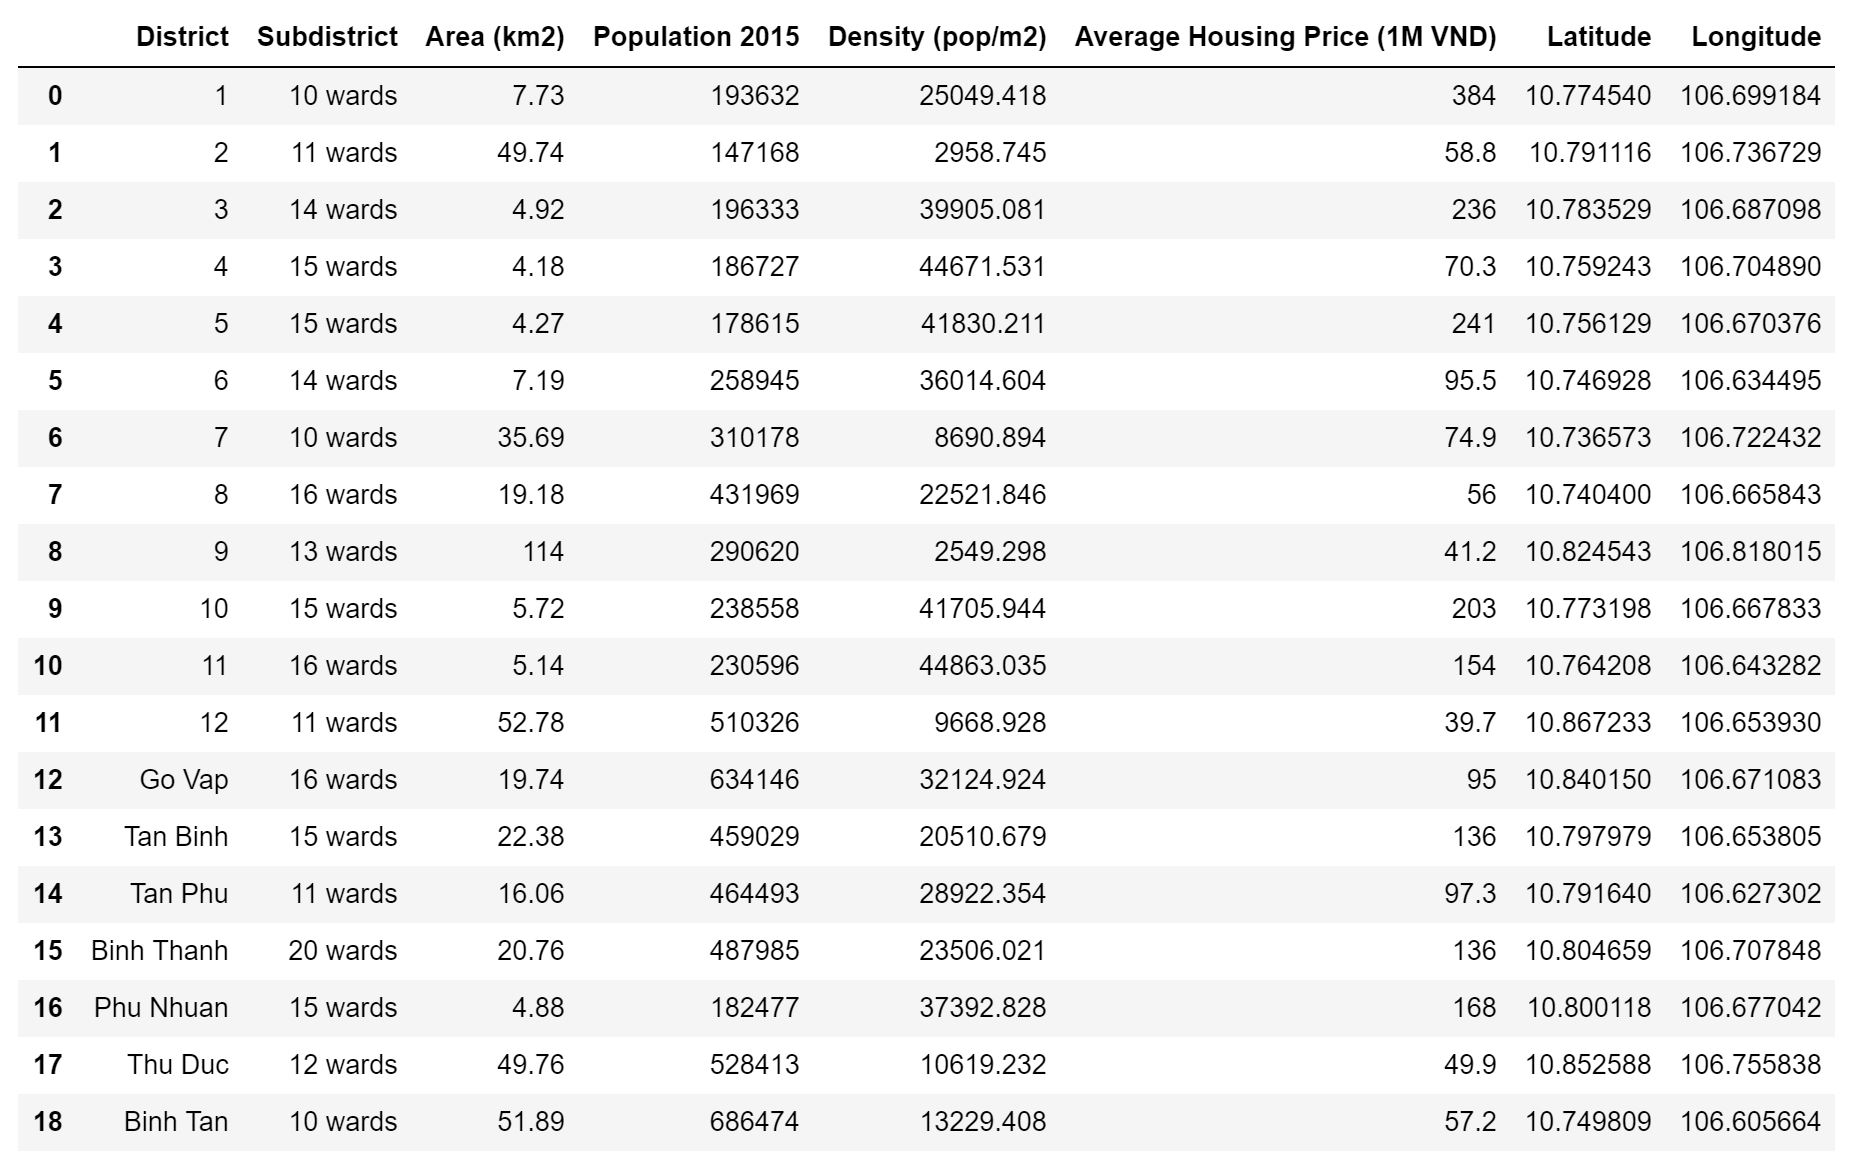
\includegraphics[width=\textwidth]{fig/df}
    \end{center}
    \caption{The main data frame.}
    \label{fig:df}
    \end{figure}
\end{center}

\subsection{Venues per  District}

We plot a chart in order to compare visually the different of number of venues between districts. This chart is shown in Figure~\ref{fig:ve-per-dis}.

\begin{center}
    \begin{figure}[htp]
    \begin{center}
     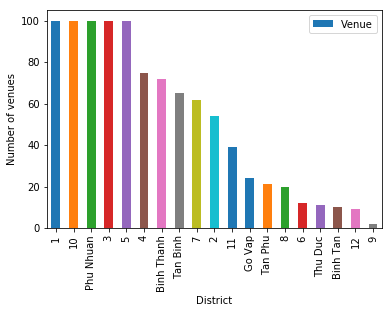
\includegraphics[width=0.7\textwidth]{fig/venues-per-district}
    \end{center}
    \caption{The number venues in each district.}
    \label{fig:ve-per-dis}
    \end{figure}
\end{center}

From this chart, we see that the districts \textbf{1, 10, 3, 5, Phu Nhuan} are the most dynamic ones. For the districts 1, 3 or 5, they are three center districts of HCMC, thus the high number of venues in these districts are not so strange. We pay attention to \textbf{Phu Nhuan} which is not a center district. We also notice on the \textbf{District 4} which has more venues than the others although in reality, who live in HCMC will think that is strange.

\subsection{Categories per District}

The chart in Figure~\ref{fig:cat-per-dis} gives us an overview of the number of categories in each district.

\begin{center}
    \begin{figure}[htp]
    \begin{center}
     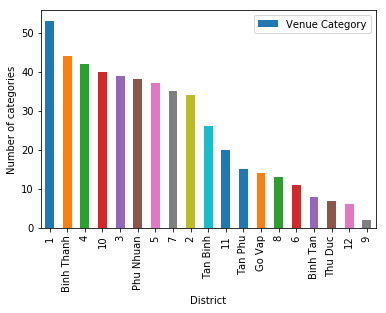
\includegraphics[width=0.7\textwidth]{fig/cat-per-dis}
    \end{center}
    \caption{The number categories in each district.}
    \label{fig:cat-per-dis}
    \end{figure}
\end{center}

Again, the district 1 wins the top. However in this time, the \textbf{Binh Thanh} runs the second instead of district 3 or 5 like in Figure~\ref{fig:ve-per-dis}. The \textbf{District 4} is still very diversity. The reason for that there are many venues but les categories in some districts is maybe there are some principle categories in these districts. Those principle categories play the major role in the commercial activities of these districts.

\subsection{Venues per Category}

Look at the most 5 categories, we have \textit{Vietnamese Restaurant} (133), \textit{Café} (127), \textit{Coffee Shop} (72), \textit{Seafood Restaurant} (33), \textit{Asian Restaurant} (29). \textbf{The café} is the main category in the drinks business with 127 different venues!

\subsection{Top 10 venue categories in each district}

Figure~\ref{fig:10-most-cat} shows us the most 10 categories in each district. For less copetition, we can choose districts whose fitst most common venue is not café. For examples, districts 1, 10, 2, 3, 4, 5.

\begin{center}
    \begin{figure}[htp]
    \begin{center}
     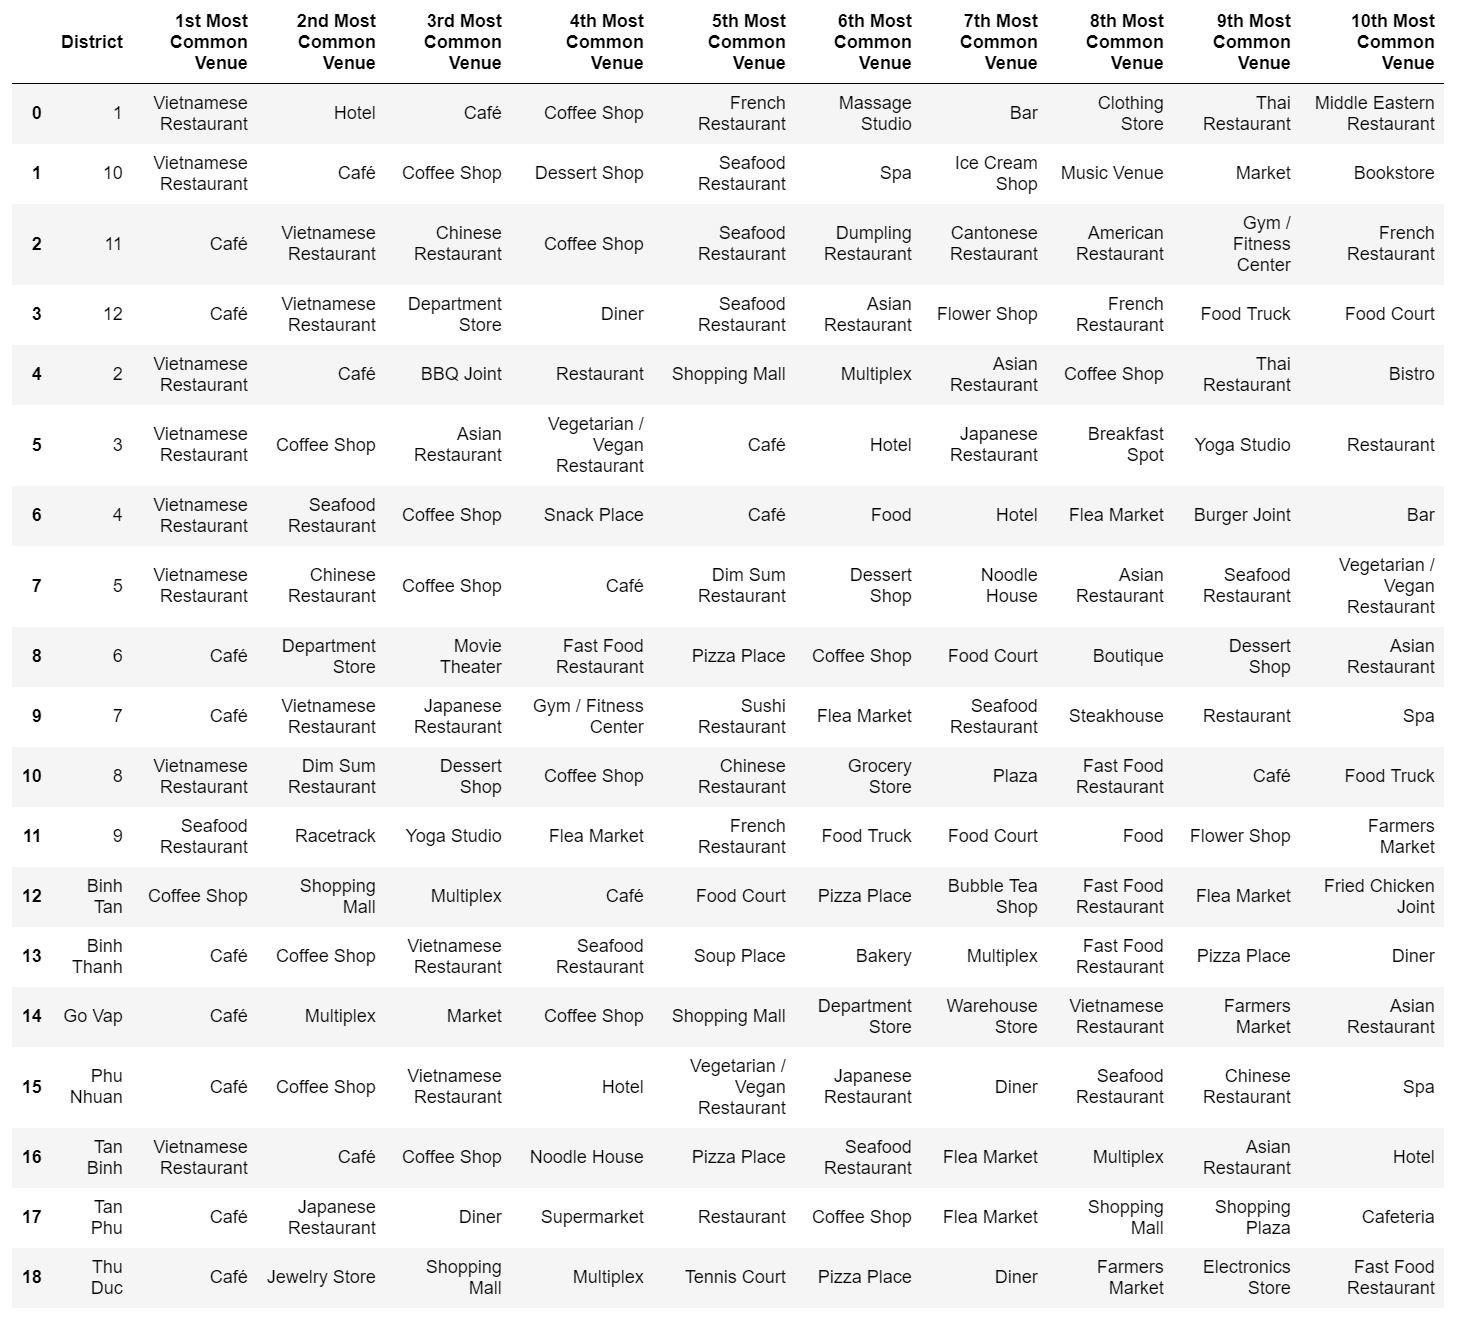
\includegraphics[width=\textwidth]{fig/df_10}
    \end{center}
    \caption{Top 10 venue categories for each district.}
    \label{fig:10-most-cat}
    \end{figure}
\end{center}

\subsection{How many clusters?}
\label{sec:cluster}

We consider the data relating to category "café" only. We want to cluster them into several groups. First, we need to determine the number of groups (or K for the K-means method). Using the elbow method with different values of K, Figure~\ref{fig:elbow} shows that \textbf{3} is the best choice.

\begin{center}
    \begin{figure}[htp]
    \begin{center}
     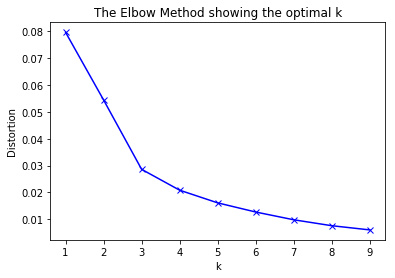
\includegraphics[width=0.7\textwidth]{fig/elbow}
    \end{center}
    \caption{The optimal number of groups/clusters.}
    \label{fig:elbow}
    \end{figure}
\end{center}

We can name the clusters like these,

\begin{itemize}
\item \textbf{Cluster 0} : There are not many café shops in these districts.
\item \textbf{Cluster 1} : There are a lot of café shops in these districts.
\item \textbf{Cluster 2} : The number of café shops in these districts is medium.
\end{itemize}

Figure~\ref{fig:cluster} illustrates the clusters of all urban districts in HCMC. With this map, we can easily distinguish the clusters between districts.

\begin{center}
    \begin{figure}[htp]
    \begin{center}
     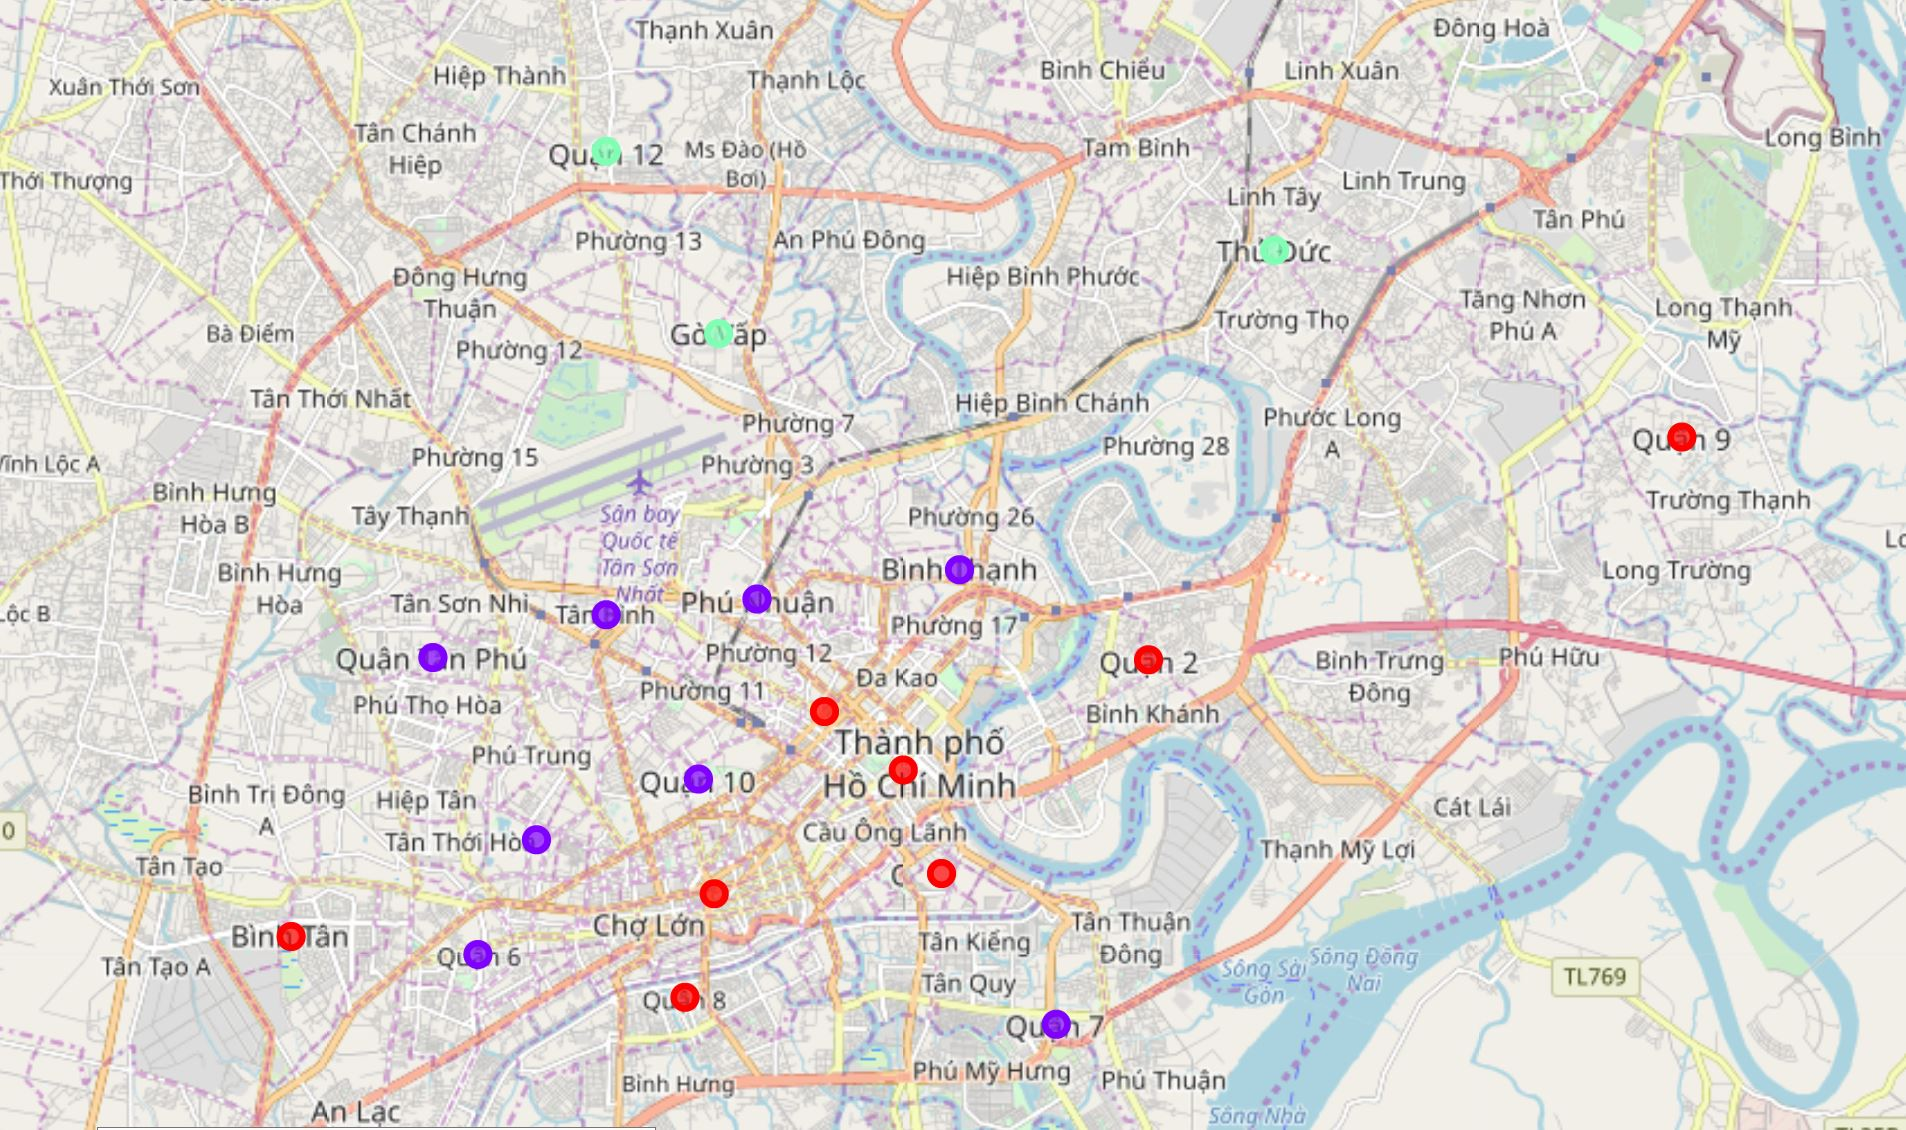
\includegraphics[width=\textwidth]{fig/cluster}
    \end{center}
    \caption{The maps of clusters. Cluster 0 (Red), Cluster 1 (Violet), Cluster 2 (Cyan).}
    \label{fig:cluster}
    \end{figure}
\end{center}

\subsection{AHP vs the number of café}

Look back to the average housing price table (AVH), we categorize them into 4 groups (unit: million VND). Figure~\ref{fig:ahp} indicates that the low price housing take the majority. We need to focus on the \textbf{Low} and \textbf{Medium} housing price to set up our business.

\begin{itemize}
\item \textbf{Low} : $30 < AHP \le 100$.
\item \textbf{Medium} : $100 < AHP \le 200$.
\item \textbf{High} : $200 < AHP \le 300$.
\item \textbf{Very high} : $300 \le AHP$.
\end{itemize}

\begin{center}
    \begin{figure}[htp]
    \begin{center}
     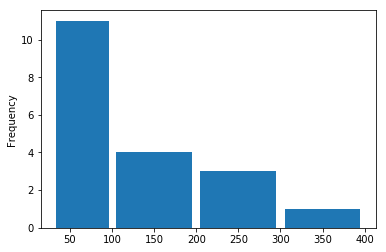
\includegraphics[width=0.7\textwidth]{fig/ahp}
    \end{center}
    \caption{The distribution of AHP.}
    \label{fig:ahp}
    \end{figure}
\end{center}

Look at Figure~\ref{fig:ahp_cluster}, we focus on: 

\begin{itemize}
\item \textbf{Low} AHP \& \textbf{not many café} (cluster 0) : district 2, \textbf{district 4}, district 8, district 9 and Binh Tan.
\item \textbf{Low} AHP \& medium number of café : district 12, Go Vap, Thu Duc.
\end{itemize}

\begin{center}
    \begin{figure}[htp]
    \begin{center}
     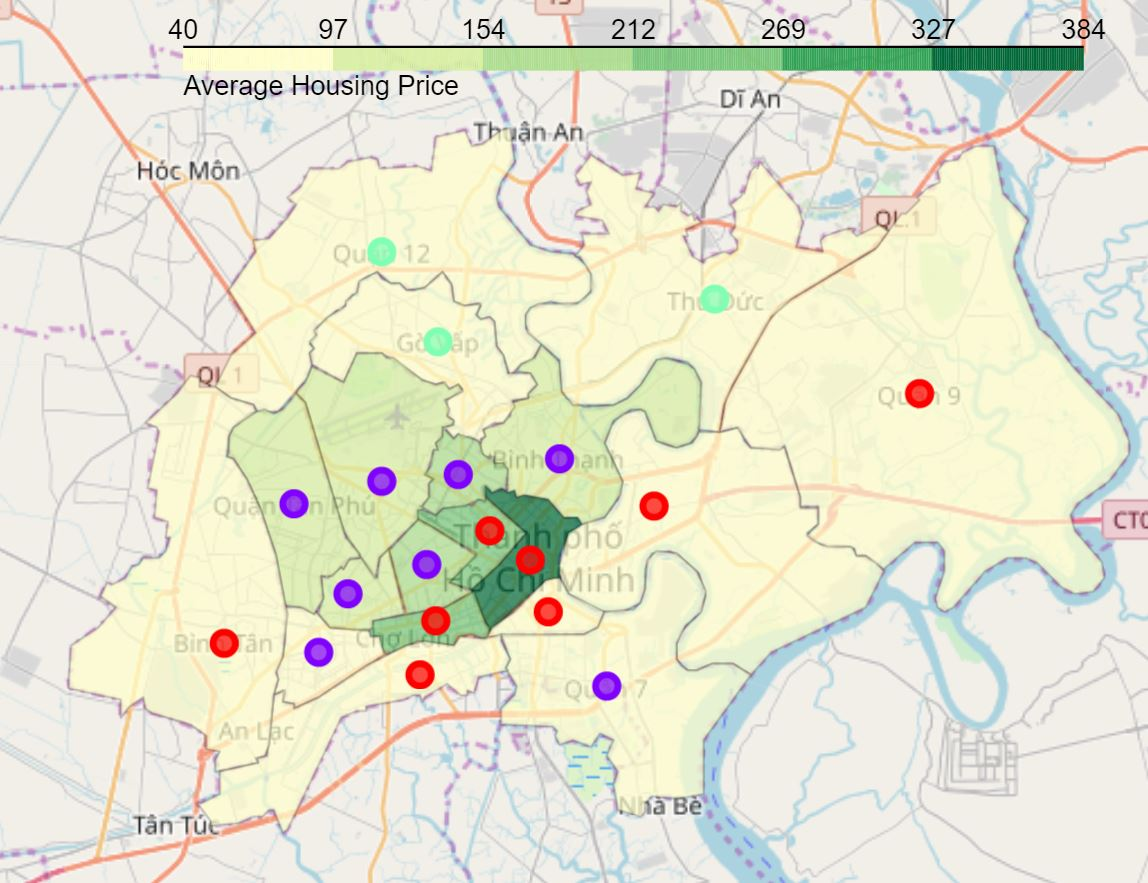
\includegraphics[width=\textwidth]{fig/ahp_cluster}
    \end{center}
    \caption{The couple maps of AHP and the clusters given in Section~\ref{sec:cluster}.}
    \label{fig:ahp_cluster}
    \end{figure}
\end{center}

\subsection{Population density vs the number of café}

We should not rely only on the relationship between AHP and clusters. For example, district 9 has almost no café and it has also very low AHP but in reality, this district contains many industry zones and there are not many people living around here. That's why we need to consider also the density of each district. Just think that, if there are not enough people to come to our café, how can we make a profit?

Figure~\ref{fig:ahp_density} gives us a full picture about the relation between population density and the clusters.

 \begin{center}
    \begin{figure}[htp]
    \begin{center}
     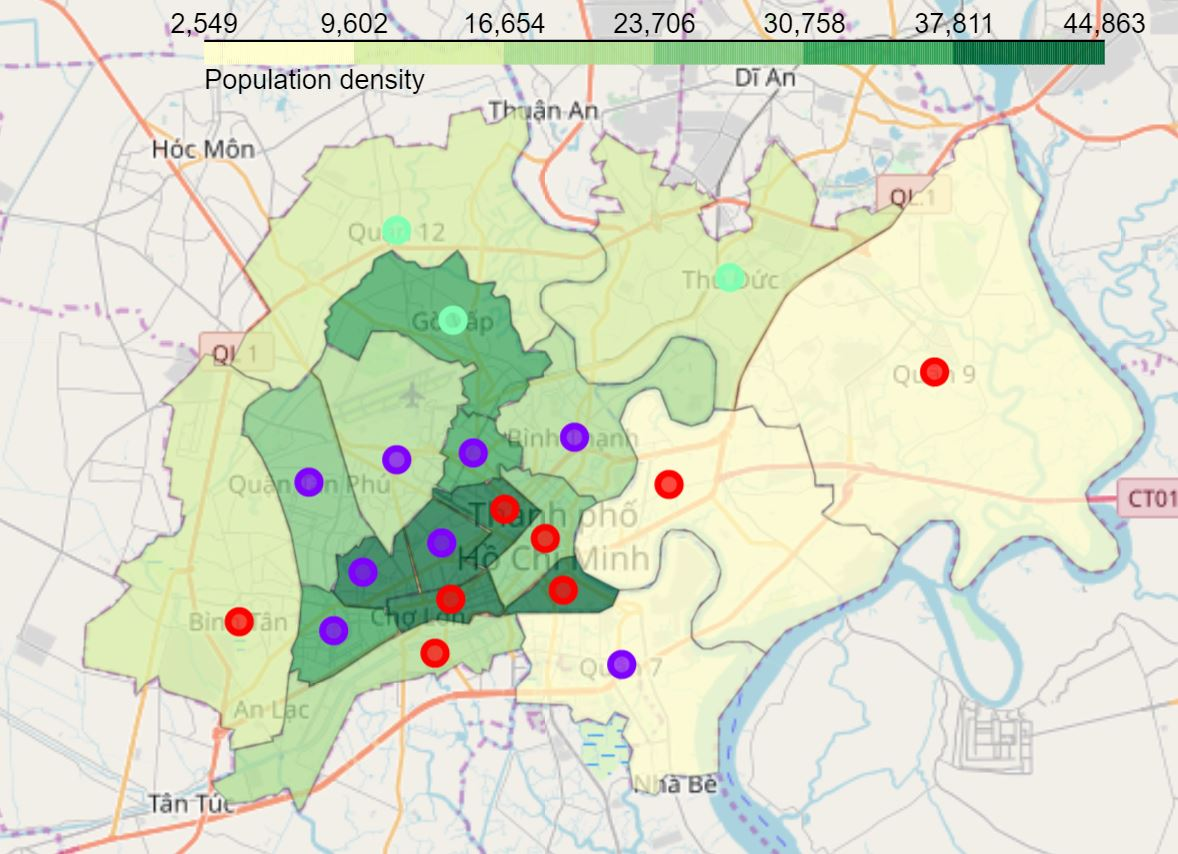
\includegraphics[width=\textwidth]{fig/ahp_density}
    \end{center}
    \caption{The couple maps of AHP and the population density of each district.}
    \label{fig:ahp_density}
    \end{figure}
\end{center}

We focus on:

\begin{itemize}
\item \textbf{High density} + \textbf{not many café} : district 3, \textbf{district 4}, district 5.
\end{itemize}

\section{Conclusion}

From all above results, we conclude that, the best place for us to set up a new café is in \textbf{district 4} because there are a lot of people living there (high density), there are not many already-working café (cluster 0) and the average housing price is low.

%\section{Discussion}



%\begingroup
%\let\clearpage\relax
%\addcontentsline{toc}{section}{References}
%\printbibliography
%\endgroup

\end{document}